% Figura cuerpo B2 (Fricciones, rigideces nominales): por qué la pérdida privada es de
% segundo orden y la social de primer orden. El panel (a) es el aparato que reutiliza b2_amplificador.
\documentclass[tikz,border=3pt]{standalone}
\usepackage[T1]{fontenc}
\usepackage[utf8]{inputenc}
\usepackage{amsmath}
\usetikzlibrary{arrows.meta,calc,positioning,decorations.pathreplacing}
\begin{document}
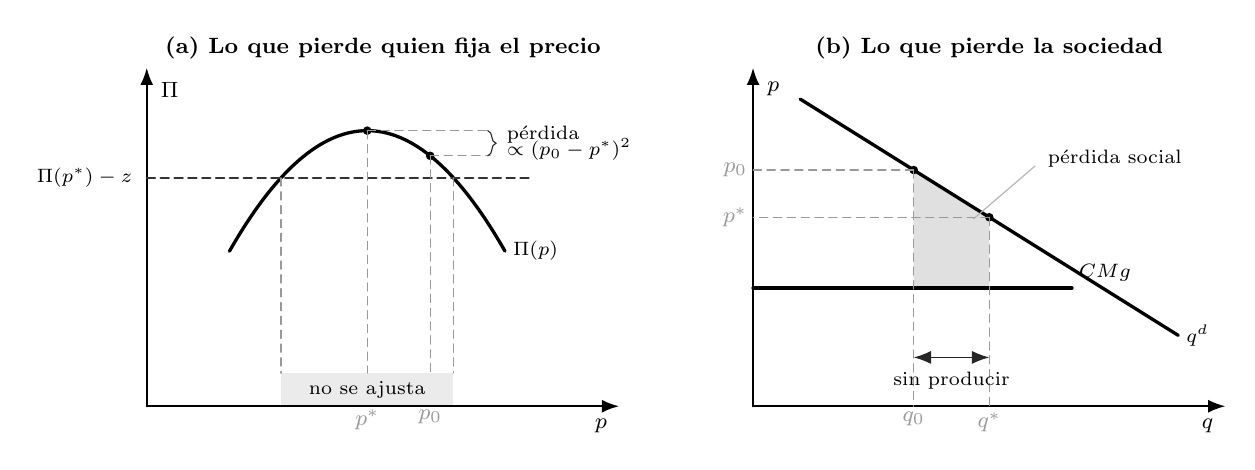
\begin{tikzpicture}[>={Latex[length=2.2mm]}, line cap=round, font=\footnotesize,
  eje/.style={->, thick},
  curva/.style={very thick},
  guia/.style={densely dashed, gray!80},
  umbral/.style={densely dashed, thick, gray!40!black},
  pto/.style={circle, fill=black, inner sep=1.1pt}]

  % ================= Panel (a): quien fija el precio =================
  \node[font=\footnotesize\bfseries] at (3.0,4.55) {(a) Lo que pierde quien fija el precio};
  \fill[black!8] (1.705,0) rectangle (3.895,0.42);
  \draw[eje] (0,0) -- (6.0,0) node[below left=1pt]{$p$};
  \draw[eje] (0,0) -- (0,4.3) node[below right=2pt]{$\Pi$};
  \draw[curva, domain=1.05:4.55, samples=80] plot (\x,{3.5-0.5*(\x-2.8)^2})
    node[right=-1pt, font=\scriptsize]{$\Pi(p)$};
  \draw[umbral] (0,2.9) -- (4.9,2.9);
  \node[anchor=east, font=\scriptsize] at (-0.06,2.9) {$\Pi(p^{*})-z$};
  \draw[guia] (1.705,2.9) -- (1.705,0.42);
  \draw[guia] (3.895,2.9) -- (3.895,0.42);
  \node[font=\scriptsize] at (2.8,0.21) {no se ajusta};
  % puntos
  \node[pto] (M) at (2.8,3.5) {};
  \node[pto] (V) at (3.6,3.18) {};
  \draw[guia] (2.8,3.5) -- (2.8,0.42) node[below=0.42cm, inner sep=1pt]{$p^{*}$};
  \draw[guia] (3.6,3.18) -- (3.6,0.42) node[below=0.42cm, inner sep=1pt]{$p_{0}$};
  % la perdida
  \draw[guia] (2.8,3.5) -- (4.36,3.5);
  \draw[guia] (3.6,3.18) -- (4.36,3.18);
  \draw[gray!30!black, decorate, decoration={brace, amplitude=3pt}] (4.33,3.5) -- (4.33,3.18);
  \node[anchor=west, font=\scriptsize, align=left] at (4.45,3.34)
    {pérdida\\[-2pt]$\propto(p_{0}-p^{*})^{2}$};

  % ================= Panel (b): la sociedad =================
  \begin{scope}[xshift=7.7cm]
    \node[font=\footnotesize\bfseries] at (3.0,4.55) {(b) Lo que pierde la sociedad};
    \fill[black!12] (2.04,1.5) -- (2.04,3.0) -- (3.0,2.4) -- (3.0,1.5) -- cycle;
    \draw[eje] (0,0) -- (6.0,0) node[below left=1pt]{$q$};
    \draw[eje] (0,0) -- (0,4.3) node[below right=2pt]{$p$};
    \draw[curva] (0.6,3.9) -- (5.4,0.9) node[right=-1pt, font=\scriptsize]{$q^{d}$};
    \draw[curva] (0,1.5) -- (4.05,1.5) node[above right=-2pt, font=\scriptsize]{$CMg$};
    \node[pto] (A) at (2.04,3.0) {};
    \node[pto] (B) at (3.0,2.4) {};
    \draw[guia] (2.04,3.0) -- (0,3.0) node[anchor=east, inner sep=2pt]{$p_{0}$};
    \draw[guia] (3.0,2.4) -- (0,2.4) node[anchor=east, inner sep=2pt]{$p^{*}$};
    \draw[guia] (2.04,3.0) -- (2.04,0) node[below, inner sep=2pt]{$q_{0}$};
    \draw[guia] (3.0,2.4) -- (3.0,0) node[below, inner sep=2pt]{$q^{*}$};
    \draw[<->, gray!30!black] (2.04,0.62) -- (3.0,0.62);
    \node[font=\scriptsize, anchor=north] at (2.52,0.56) {sin producir};
    \node[anchor=west, font=\scriptsize, align=left] at (3.62,3.15) {pérdida social};
    \draw[gray!60] (3.58,3.05) -- (2.80,2.38);
  \end{scope}
\end{tikzpicture}
\end{document}
